%-------------------------------- Configurações --------------------------------

\documentclass[
  a4paper,         % Tamanho do papel: A4
	abntfigtabnum,
  noindentfirst,
	normaltoc,
	pnumplain,
	notimes
	% capchap,
]{abnt}

\usepackage[utf8]{inputenc}
\usepackage[brazil]{babel}
\usepackage{url}
\usepackage{graphicx}
\usepackage{enumerate}
\usepackage[pdfborder={0 0 0}]{hyperref} % http://www.tug.org/applications/hyperref/manual.html
\usepackage[alf]{abntcite}
\usepackage{listings} % http://www.atscire.de/index.php?nav=products/listings2 http://linorg.usp.br/CTAN/macros/latex/contrib/listings/listings.pdf
\usepackage{textcomp}
\usepackage[usenames,dvipsnames]{xcolor} % http://en.wikibooks.org/wiki/LaTeX/Colors
\usepackage[algoruled,longend]{algorithm2e}
\usepackage{mathtools, mhsetup} % fórmulas matemáticas
\usepackage[usenames,dvipsnames]{pstricks} % gerar os gráficos
\usepackage{epsfig} % gerar os gráficos
\usepackage{float} % dependência do H para posição
\usepackage[all,cmtip]{xy}

\urlstyle{same} % http://en.wikibooks.org/wiki/LaTeX/Hyperlinks#Customization

%-------------------------------- Highligthing ---------------------------------

\lstset{
    language=C,
    basicstyle=\footnotesize\ttfamily,
    columns=flexible,
    numberbychapter=false,
    showstringspaces=false,
    tabsize=2,
    xleftmargin=17pt,
    framexleftmargin=17pt,
    framexrightmargin=5pt,
    framexbottommargin=4pt,
    numbers=left,
    numberstyle=\scriptsize\ttfamily\color{Gray},
    emphstyle=\color{OrangeRed},
    commentstyle=\color{Gray}\textit,
    stringstyle=\textit,
    keywordstyle=\textbf,
    morekeywords={@self, @caller, @const, @local},
    % emph={[2]Funcionalidade, Como},
    % emphstyle=[2]\color{MidnightBlue},
}

\usepackage{caption}
\DeclareCaptionFont{white}{\color{white}\footnotesize\bfseries}
\DeclareCaptionFormat{listing}{\colorbox{BrickRed}{\parbox{\textwidth}{#1#2#3}}}
\captionsetup[lstlisting]{format=listing,labelfont=white,textfont=white}

% Renomear listing e listings -> código e códigos
\renewcommand*\lstlistingname{Código}
\renewcommand*\lstlistlistingname{Lista de Códigos}
\graphicspath{graficos/}

%--------------------------------- Informações ---------------------------------

\begin{document}

\titulo{Gração de perfis de usuário para mineração de uso}
\autor{Rafael Barcellos Pessanha Crespo}
\instituicao{Universidade Estadual do Norte Fluminense Darcy Ribeiro}
\orientador[Tutor: ]{Luis Antonio Rivera Escriba.}
\comentario{Monografia apresentada ao Curso de Graduação em Ciência da
Computação da Universidade Estadual do Norte Fluminense Darcy Ribeiro como
requisito para obtenção do título de Bacharel em Ciência da Computação, sob
orientação do Profº. Luis Antonio Rivera Escriba.}
\local{Campos dos Goytacazes/RJ}
\data{2012}

\graphicspath{{graficos/}}
\capa
\folhaderosto

\sumario

\chapter{Introdução}

\section{Introdução}
    A Mineração Web é uma metodologia de recuperação da informação, que usa ferramentas de mineração de dados para extrair informações tanto do conteúdo das páginas da internet e de sua estrutura de relacionamentos (links), quanto dos registros de navegação dos usuário.

	Este segmento da mineração vem chamando a atenção principalmente das empresas de e-commerce nos últimos anos, pois tem sido visto como uma grande arma para “conhecer” seu cliente, que neste caso é o usuário que está navegando no site. Essas empresas visam investir em pesquisa e desenvolvimento de métodos de mineração para aplicar essa prática e assim conseguir reverter os dados obtidos ao seu favor, direcionando para uma estratégia de marketing mais eficaz, por exemplo.

	Todas as empresas que vendem produtos ou serviços, dependem de sua fama e de seus clientes, portanto uma boa relação entre a empresa e o cliente é de extrema importância para que este torne-se fiel à determinada empresa, o problema é que com a globalização, que trouxe à tona os serviços remotos, como vendas online e pelo telefone, veio junto uma maior dificuldade de entender e “analisar” o comportamento do cliente, saber o que ele procura, qual a abordagem utilizar, o que oferecer, já que agora este não está mais fisicamente presente, ou seja, não há um contato direto entre vendedor e cliente, e é a partir deste problema que a mineração web passa a ser uma ferramente essencial.

\section{Objetivos e justificativas}

\begin{itemize}
\item Item 1
\item Item 2
\item Item 3
\end{itemize}


\section{Estrutura do trabalho}


\chapter{Mineração Web}
A mineração web utiliza muitos conceitos da mineração de dados tradicional, por isso para começarmos a falar do assunto principal deste trabalho, que é a Mineração Web, teremos que introduzir alguns termos e conhecimentos mínimos de entendimento necessário para facilitar a compreensão.

\section{Mineração de Dados}

	Segundo Liu\cite{BingLiu}, Mineração de Dados ou Data mining é o processo de analisar um grande conjunto de dados com o objetivo de encontrar padrões, informações relevantes para algum propósito de interesse da instituição ou empresa. Devido à grande quantidade de dados que existem hoje em dia, geralmente não é mais possível fazer a análise individual dos dados para então obter-se alguma informação. Para solucionar esse problema, utilizamos a mineração de dados  que é capaz de fazer essa análise em uma grande quantidade de dados. A mineração de dados é uma iteração das seguintes etapas:

\begin{itemize}
\item 	Pré-processamento: nesta etapa é feita uma preparação dos dados recolhidos, ou seja, os dados são analisados e ruídos são retirados, pois geralmente não estão devidamente adequados para mineração logo após o recolhimento;
\item 	Mineração: após o pré-processamento o dado será então minerado pelo algoritmo que produzirá padrões e conhecimentos;
\item  	Pós-processamento: para finalizar é feita a identificação e seleção dos padrões úteis para a pesquisa, já que muitas vezes os padrões encontrados pelo algoritmo não são úteis.
\end{itemize}

Apesar de utilizar muitos fundamentos da mineração de dados tradicional, existem algumas diferenças entre esta e a mineração web, sendo a principal delas é que a primeira aplica a mineração em dados estruturados, organizados em tabelas, como em um banco de dados, e a segunda em dados não-estruturados ou semi-estruturados.


\section{A Mineração Web}
	Segundo Liu\cite{BingLiu}, web mining é o uso das técnicas de data mining para descobrir e extrair automaticamente informações relevantes dos documentos e serviços ligados a internet.

	Este tipo de mineração utiliza as técnicas de data mining, com algumas modificações já que os dados na web não são estruturados, para extrair automaticamente informações relevantes dos documentos e serviços ligados à intenet, e sua aplicação pode ter os seguintes objetivos: encontrar documentos, (encontrar sites na web contendo documentos especificados por palavras-chave), selecionar e pré-processar informações, generalizar (descobrir padrões gerais entre sites), validar e interpretar os padrões minerados.

	Apesar de ter como base a mineração de dados, a mineração web desenvolveu muitas formas próprias de mineração, devido à grande variedade de informações e dados que são disponibilizados na internet.

	A Mineração Web hoje tem se tornado cada vez mais importante e mais estudada, e isto se deve por alguns fatores: o crescimento significativo de dados e informações lançadas na rede, a grande variedade de tipos de dados, a heterogeneidade das informações, ou seja, grande quantidade de sites, blogs que abordam um mesmo assunto e portanto geram informações similares, no entanto com um vocabulário totalmente diferente um do outro, o que dificulda muito a integração dessas informação.

	Existem alguns fatores que facilitam a análise de uma página, tanto positivamente, quanto negativamente, por exemplo, um site  que tem seu link referenciado por muitas vezes em vários outros sites, pode ser considerado um site com informações de qualidade e ao mesmo tempo confiável, já um site que tem muita informação espalhada, conteúdo principal, links, propagandas, etc, já é mais difícil de ser analisado, logo também será mais difícil de recolher informações relevantes dele. Um dos motivos pelo qual a web é fonte de tanta informação e tem se tornado cada vez mais, é a facilidade com que as pessoas podem gerar conteúdo e publicar na internet, a consequência dessa facilidade é uma enorme quantidade de informações erradas, incompletas ou até mesmo mentirosas.

	A internet é muito dinâmica, as informações estão em mudança constante, esse dinamismo também é refletido na maneira de analisar os dados oriundos da web, a cada momento são criadas novas formas de mineração, por exemplo, mineração de opinião, que é um tipo de mineração que analisa as informações postadas em fóruns por clientes, que fazem um relato sobre algum outro site ou sobre algum serviço ou produto utilizado; análise de redes sociais, que hoje em dia é uma fonte inesgotável e incessante de informações, pois os usuários estáo gerando conteúdo a todo instante, comentando sobre serviços, notícias, sobre qualquer coisa, e muitas dessas informações postadas nas redes sociais são de extrema importância para os interessados, por exemplo a empresa que realizou o serviço ou a venda para tal usuário.

	Existem três categorias de mineração web e elas são divididas de acordo com a parte da Web a ser analisada como mineração de estrutura, mineração de uso e mineração de conteúdo. Ver Figura 1.

\begin{figure}[!htb]
\centering
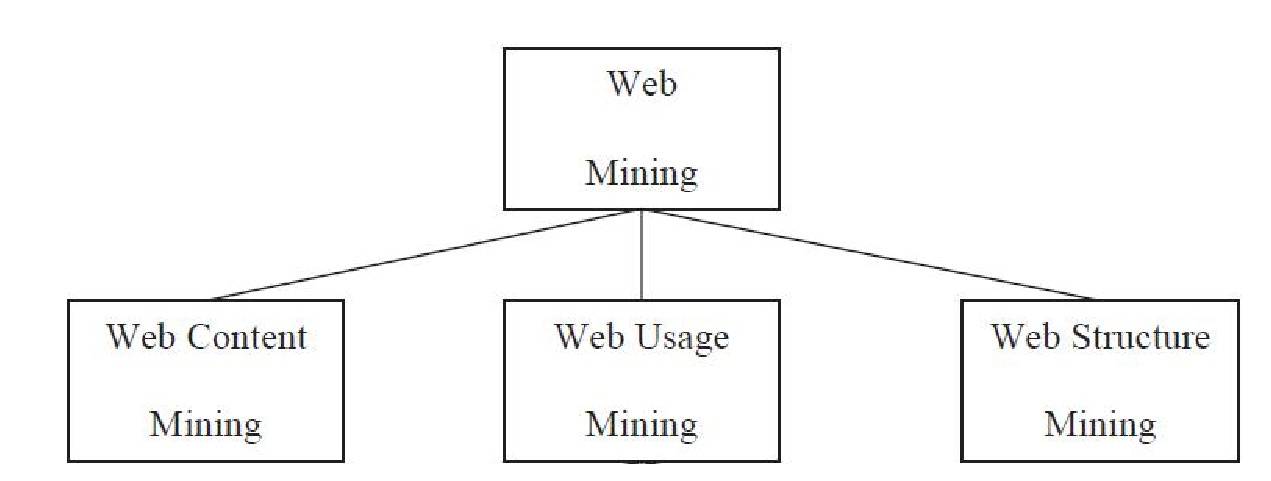
\includegraphics[scale=0.5]{categorias}
\caption{Ramificação das principais categorias da Mineração Web}
\label{Rotulo}
\end{figure}

\subsection{Mineração de Estrutura}

	De acordo com Kosala\cite{Kosala}, o foco da mineração web de estrutura (Web Structure Mining) é na estrutura dos hiperlinks dentro da própria Web. Esta categoria de mineração utiliza a estrutura de hiperlins da Web para aplicar a análise de redes sociais para modelar a estrutura de links da Web.

	Para tentarmos entender um pouco melhor, pensemos na Web como um grafo, onde as arestas são os links entre as páginas e os nós são as próprias páginas.

	A mineração de estrutura utiliza a teoria de grafos para analisar a estrutura de nó e conexão  de um site web. Este tipo de mineração descobre informações úteis dos links, que representam a estrutura da web. Por exemplo, através dos links nós podemos encontrar páginas importantes, que são a chave tecnológica usada nos motores de busca, podemos tambem encontrar comunidades de usuários com interesses em comum. O principal objetivo deste tipo de mineração é extrair relações previamente desconhecidas entre as páginas da web.

	Este modelo é usado para classificar páginas da Web a respeito da similaridade ou relação existente entre elas. Através dessa análise podemos descobrir sites de autoridade ( sites que tem seus links frequentemente citados em outros sites).

\subsection{Mineração de Conteúdo}
    Kosala\cite{Kosala} considera que a Mineração Web de conteúdo (Web Content Mining) concentra sua atenção sobre os padrões de exploração e produção dos objetos disponíveis na Web, como arquivos HTML, imagens, e-mails, bancos de dados on-line, etc., permitindo a descoberta de palavras-chave, frases e informações interessantes sobre esses objetos, facilitando a avaliação, identificação, recuperação de dados e documentos, etc.

	Este tipo de mineração extrai informações úteis do conteúdo de uma página web. É possível classificar e agrupar páginas da web pelo seu conteúdo, o que é uma técnica do método tradicional da mineração de dados, mas também podemos descobrir padrões, e extrair dados úteis deles. Focando a análise para a relação cliente-empresa, podemos extrair opiniões dos clientes para saber o que pensa o consumidor.

	A mineração de conteúdo engloba os textos, imagens, vídeos, sons (que também é chamada de Mineração de Dados Multimídia) , hiperlinks; ou seja, é uma análise que busca informações em diversos tipos de dados.  Apesar de analisar vários tipos de arquivos, seu foco principal é na análise de textos e hipertextos. Esta área do web mining utiliza muito o Text Mining para poder obter informações dos textos não estruturados encontrados na rede.

	Quando falamos de Mineração de Conteúdo, podemos aborda-la de duas maneiras:

\begin{itemize}
\item 	Recuperação de Informação: tem o objetivo de auxiliar o usuário na busca de informação, usado nos principais mecanismos de buscas da internet, através da utilização de palavras-chave.
\item 	Banco de Dados: tem o objetivos de organizar os dados Web para que possam ser feitas contultas mais sofisticadas, e não sejam apenas buscas de palavras-chave.
\end{itemize}

\subsection{Mineração de Uso}

    De acordo com Jeria\cite{Escobar}, a Mineração Web de Uso se trata da aplicação de técnicas de mineração para descobrir padrões de uso da informação Web com o objetivo de entender e satisfazer as necessidades dos usuários. Para este ramo da Mineração Web a principal fonte de informações são os arquivos de log dos servidores Web.

	Enquanto a mineração de conteúdo e a mineração de estrutura utilizam os dados reais ou primários da Web, a mineração de uso lida com os dados secundários, que são gerados a partir da interação do usuário com a Web. Os dados de uso da Web incluem informações de logs de servidores web, logs de servidores proxy, logs de browsers, perfis de usuário, cookies, seções ou transações de usuários, pasta de favoritos, consultas do usuário, cliques de mouse e qualquer outro dado gerado pela interação do usuário com a Web.\cite{Girardi} O objetivo principal é capturar, modelar e analisar o padrão de comportamento e os perfis dos usuários que interagem com o Sistema.

	Com o aumento constante da popularidade e do uso do e-commerce, o número de cliques e as transações de dados coletadas da web alcançaram proporções enormes.

	Analisar tantos dados ajuda as organizações a determinar o tempo de vida dos clientes, a criar estrategias de marketing de produtos e serviços, avaliar o efeito das promoções, providenciar mais conteúdo personalizado para clientes.

	Os padrões descobertos geralmente são recursos frequentemente acessados por grupos de usuários com interesses em comum.

	Na próxima seção deste texto faremos uma explanação mais detalhada desta categoria de mineração, que é o foco principal deste trabalho.

\section{Mineração de uso Web}
    De acordo com \cite{Girardi}, o processo de mineração de uso da Web pode ser classificado segundo duas abordagens. Uma delas mapeia os dados de uso do servidor Web em tabelas relacionais antes das técnicas adaptadas de mineração de dados serem aplicadas. A outra utiliza os dados de logs diretamente utilizando técnicas especiais de pré-processamento. Assim como no KDD, que é um processo de descobrimento de conhecimento a partir de um grande volume de dados, a limpeza e pré-processamento dos dados, aqui, é uma parte crucial do processo, pois a qualidade desses dados vai determinar a eficiência dos algoritmos de mineração.

	A mineração de uso é dividida em uma sequência de três etapas principais: colheita de dados e pré-processamento, descoberta de padrão e análise do padrão, como é ilustrado na Figura 2.

\begin{figure}[!htb]
\centering
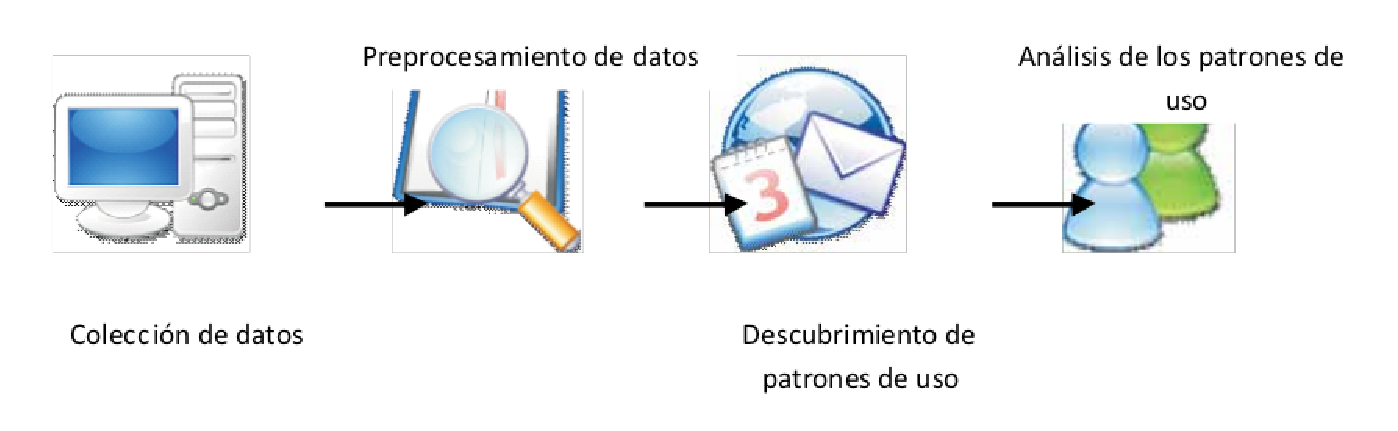
\includegraphics[scale=0.7]{grafico3}
\caption{Etapas da mineração de uso}
\label{Rotulo}
\end{figure}

\begin{enumerate}[A)]
\item Coleção de dados:
    O uso da web implica em uma variedade muito grande de fontes de informações, como por exemplo:
\begin{itemize}
\item 	Log de servidor Web: que armazena as informações de acesso nos registros de serviço de acesso (log). Para cada sessão de navegação são guardados os arquivos de registro de serviço de acesso (log), que armazena dados de acesso como IP, data de acesso, transferencia de bytes, etc; log de erros, que armazena informações das falhas de requisição do cliente e log de cookies, que guarda a informação de acesso da sessão entre o cliente e o servidor.
\item Log de servidor proxy: que pode ser usado como fonte de dados para caracterizar o comportamento de navegação do usuário.
\item Log da máquina do cliente: se encontram na máquina do cliente e são encarados como o melhor tipo de dado para revelar os padrões de navegação de um usuário. Onde ficam os cookies que armazenam e ao mesmo tempo fornecem informações para os servidores web.
\end{itemize}

\item Pré-processamento:

	 Nesta etapa os fluxos de cliques são limpos, ou seja, é feito um refinamento dos cliques, reduzindo ao máximo os cliques falsos e irrelevantes para a busca, e particionados em conjuntos de transações que representarão as atividades de cada usuário durante várias visitas ao site. Outros critérios como o conteúdo e a estrutura do site também podem ser usados no pré-processamento para melhorar a transação de dados do usuário.

	É importante criar o conjunto de dados alvo adequados para aplicar a mineração e os algoritmos de estatística, por causa da característica dos dados do fluxo de cliques e a sua relação com os outros dados coletados.

	Geralmente esta é a etapa que consome mais tempo e processamento computacional além de  algumas vezes precisar de algoritmos e heuristicas um pouco mais sofisticadas. Este processo é crítico para o sucesso da descoberta do padrão dos dados e também pode ser chamado de preparação de dados.

	O sucesso da aplicação de técnicas de mineração de dados em Web Usage Mining é altamente dependente da aplicação correta das tarefas de pré-processamento, pois com dados bem preparados a aplicação da mineração tem uma maior probabilidade de obter melhores resultados, já que terá menos ruído em seu caminho.

\item Descoberta do padrão:
	Nesta etapa são usadas as estatísticas e base de dados, além da realização de operações de máquinas de aprendizagem para obter os padrões que estão escondidos, ocultos, que refletem no comportamento padrão dos usuários.

    É nessa fase que os algoritmos de mineração vão descobrir novo conhecimento em cima do que já existe. Um exemplo que nos daria uma idéia de como seria uma saída de um desses algoritmos é:
    \begin{itemize}
    \item 70/100 das pessoas que acessam a seção de skate também acessam a seção sobre surf.
    \end{itemize}
    Neste exemplo o resultado poderia dar uma indicação ao gerente da loja virtual sobre as preferências e perfis de seus clientes, de forma a montar estratégias de vendas que possam induzir o usuário a comprar mais.

    Segundo Marinho et al.\cite{Girardi}, o maior problema em aprender ou descobrir novos conhecimentos da Web é a falta de marcação semântica das informações, pois muitos algoritmos de mineração de dados precisam ter como referência algum conceito de positivo ou negativo do assunto. Se tivéssemos algum conjunto de páginas Web marcadas como positivas ou negativas, o trabalho de mineração seria facilitado.

    Uma das soluções deste problema de mineração é a utilização agrupamentos (clustering), que é uma técnica de classificação que não necessita de marcações semânticas, e por isso tem sido aplicada com sucesso em grandes conjuntos de documentos HTML \cite{Cutting}. Nesta técnica, os documentos são agrupados de acordo com a sua similaridade, logo, um novo documento é classificado baseado na sua similaridade com um outro documento já existente.

    Outra solução seria a utilização de \textbf{regras de associação}, que segundo \cite{Castano} é basicamente uma proposição probabilística de certos estados em uma base de dados, e podem seria representadas da forma Se X então Y, ou $ X \Rightarrow Y$, onde X e Y são conjuntos de itens e $X \cap Y = \emptyset$. $ X \Rightarrow Y$ expressa que toda vez que uma transação T contiver X então ela provavelmente também conterá Y. A probabilidade ou \textbf{confiança} da regra é a porcentagem de transações contendo Y junto a X comparado ao total de transações contendo X. A idéia de minerar regras de associação se origina nos dados de super-mercados e afins onde regras como “O cliente que compra o produto X também comprará o produto Y com probabilidade (confiança) de $p$\% ”\cite{Pal}

    Esta técnica é muito utilizada para conhecer as rotas de visitas seguidas pelos usuários das páginas Web, para poder assistir a estruturação das páginas no servidor.

\item Análise de padrão:
	Na última etapa análise de padrão, as estatísticas e os padrões encontrados na etapa anterior serão processados e filtrados para gerar um modelo de usuários agregados que poderão ser utilizados como entrada de dados para ferramentas de visualização e análise de Web, geração de relatórios ou mecanismos de recomendação.

\end{enumerate}

\subsection{Aplicações de Mineração de uso Web}
    A Mineração de uso da Web pode ter várias aplicações, isto é, dependendo de como for aplicada e quais dados estejam sendo buscados, o resultado da análise pode ser utilizado de várias maneiras diferentes, algumas das principais aplicações são: a Personalização; o Melhoramento do Sistema; a Modificação do site; a Inteligência de Negócios e a Caracterização de uso, a figura 3 ilustra um pouco estas ramificações.

\begin{figure}[!htb]
\centering
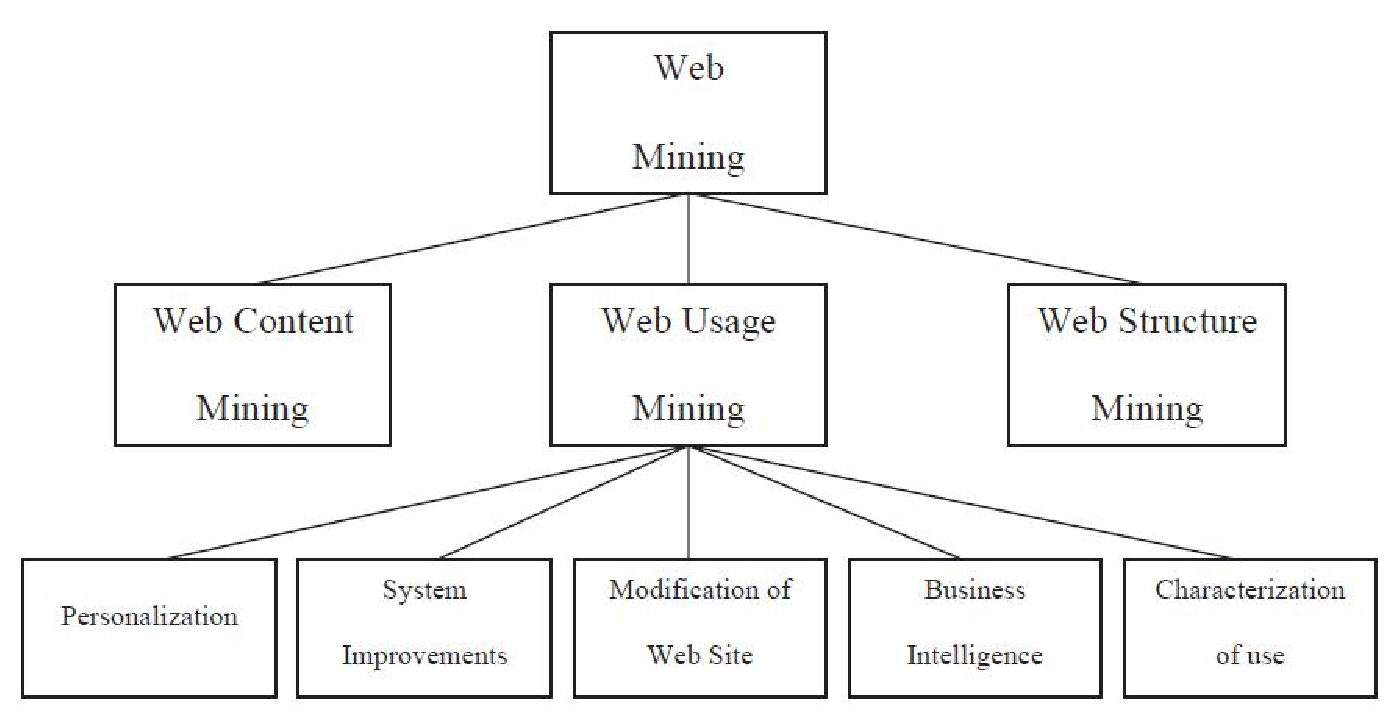
\includegraphics[scale=0.7]{aplicacoes}
\caption{Principais aplicações da mineração de uso web}
\label{Rotulo}
\end{figure}

A) \textbf{Personalização:}
    Personalizar sites é um campo de grande grande desafio, muitas pesquisas tem como objetivo utiliza-la para realizar um marketing individual para o comércio eletrônico ou até mesmo fazer recomendações dinâmicas para os usuários baseado no seu perfil e comportamento de uso.

    Jeff Bezos, CEO da Amazon.com uma vez disse: Se eu tenho 3 milhões de clientes na Web, então eu deveria ter 3 milhões de lojas na Web \cite{Schafer}, ou seja, aplicando a personalização Bezos gostaria que cada usuário acessasse uma página diferente, com ofertas e produtos que fosse adaptados de acordo com as necessidades ou características de cada um.

    Shafer\cite{Schafer} dividia este processo em duas etapas: Aprendizado e Uso. Na primeira delas é feita uma análise de dados e depois a construção do modelos de comportamento do usuário, e na etapa seguinte aplica-se o modelo a diferentes situações.

    Como foi falado anteriormente, recomendações dinâmicas podem ser feitas para o usuário, este é um tipo de personalização existente. Ele não muda apenas a forma de apresentar os dados para o usuário, mas decida quais dados ou produtos serão mostrados. Alguns métodos de recomendação são: recuperação simples, consulta feita com o usuário; itens associados, aqueles que são descobertos por análise assiciativa de vendas cruzadas; filtragem colaborativa, que a partir de um item comum, recomenda outros frequentemente vistos ou comprados por outros clientes.

B) \textbf{Melhoramento de sistemas:}
    Performance e qualidade de serviço são atributos cruciais para a satisfação do usuário. A mineração de uso gera a chave para a compreensão do comportamento do tráfego web, que pode ser usada para políticas de web caching, transmissão de rede ou distribuição de dados. A segurança na web tem sido um fator de muito interesse dos usuários, principalmente com a continuação do crescimento de comércios eletrônicos.

C) \textbf{Modificação do site:}
    A aparência de uma página web hoje, mais do que nunca é fundamental para as aplicações, principalmente quando se trata de negócios online. A mineração de uso gera um retorno detalhado do comportamento do usuário, trazendo para o web designer informações relevantes sobre mudanças que podem ser feitas na arquitetura ou no conteúdo do site. Esta é uma forma de estar sempre avaliando a usabilidade do site, pois frequentemente terá um retorno com informações recolhidas de seus usuários.

D) \textbf{Inteligência de negócios:}
    Mineração de uso Web também auxilia na forma de lidar com a inteligência de negócios, ou seja, marketing, propaganda, etc.

E) \textbf{Caracterização de uso:}
    Este método de aplicação nada mais é do que um modelo que determina as páginas que um determinado usuário deveria visitar em um site.

\section{Trabalho Relacionados}
    Nesta parte do trabalho serão destacados alguns outros trabalhos que já foram realizados por estudandes, pesquisadores, etc, e tem seu tema relacionado com o assunto que está sendo abordado pelo trabalho presente.

    Cho et al.\cite{HoCho} desenvolveram um trabalho voltado para a área de aplicação de recomendações personalizadas, onde ele desenvolve um sistema de recomendações. Inicialmente as características do usuário são recolhidos pelo rastreamento de cliques (mineração de uso); em seguida para evitar recomendações ruins que afastarão clientes, o sistema seleciona aqueles que geralmente compram produtos recomendados pelo site usando uma árvore de indução e para finalizar, medidas são elaboradas para escolher produtos mais eficientes entre os produtos candidatos.

    Já em \cite{Carmona}, a mineração de uso web é aplicada com a finalidade de ajudar ao webmaster da empresa a melhorar o design do site oroliversur.com. No trabalho a técnica de regra de associação é utilizada. Depois de realizar todo o estudo, \cite{Carmona} chegou a conclusão de que era importante prestar atenção nos acessos que eram gerados através de referências de outros sites, pois os usuários visitam um número muito baixo de páginas; e que a maioria dos acessos que eram feitos ao site eram oriundos de usuários que utilizavam o Internet Explorer como navegador. Graças a este estudo o webmaster tem agora um caminho para seguir e executar o seu trabalho seguindo informações concretas, uma das suas ações deveria ser se preocupar em fazer um layout mais otimizado para o IE.

    \cite{Zang} descreve em seu trabalho um conjunto de ferramentas que exploram dados de uso da web, ferramentas tais que identificam padrões de navegação na internet. A partir dos dados minerados pelas ferramentas, os padrões identificados são usados para alimentar a recomendação personalizada de produtos para vendas online. O objetivo principal do trabalho é mostrar que ao utilizar a rede neural de Kohonen treinada para trabalhar offline, o problema de escalabilidade, que assombra esses sistemas, seria resolvido.


\chapter{Modelo do trabalho}

    Neste capítulo será definido como será feita a coleção dos dados, quais serão os tipos de dados que serão coletados e qual será o tipo de aplicação da mineração de uso que sera utilizada.

    Os usuários da internet estão deixando rastros a todo momento enquanto navegam pela web, esses rastros são as informações que serão coletadas para serem processadas e analisadas para a geração dos perfis de usuários e padrões de uso.

    Para que o objetivo deste trabalho seja alcançado, é necessário que seja feito um estudo para que a escolha de quais serãos as informações que deverão ser retiradas dos rastros deixados pelo usuário, pois dependendo da necessidade, deve ser utilizada um tipo de informação diferente e para que os perfis coletados tenham uma certa riqueza de informações para que seja possível fazer uma boa análise de perfis, é preciso que a coleta seja feitas com foco nos rastros corretos.

\begin{figure}[!htb]
\centering
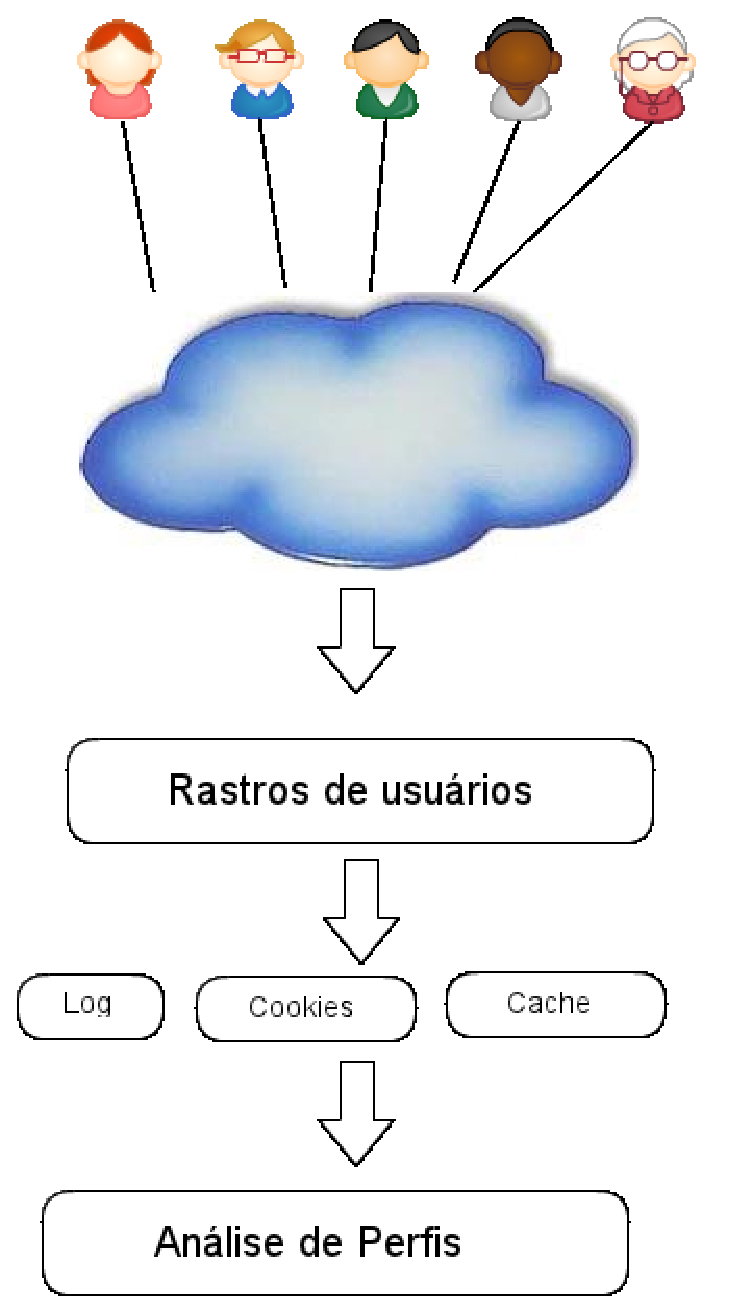
\includegraphics[scale=0.7]{diagrama}
\caption{Fluxo de informações dos usuários}
\label{Rotulo}
\end{figure}



%--------------------------------- Bibliografia --------------------------------

\citeoption{abnt-repeated-author-omit=yes}
\bibliographystyle{abnt-alf}
\bibliography{bibliografia}

\end{document}

